
\section{Introduction}

Analysing business processes based on event logs extracted from information 
systems through process mining techniques~\cite{Aalst16} becomes increasingly 
popular in industry. It enables organizations to optimize their processes and 
achieve their strategic goals, e.g., realizing cost-efficient process 
execution. However, 
%The rapid adoption of process mining 
%in industry is due to the tremendous potential of the technology. 
in practise, many business processes are not restricted to a single 
organization, but are executed by several collaborating organizations. 
We call such processes inter-organizational business processes.
An example of such a process is given in  
\autoref{fig:ground_handling_process}, which illustrates the ground handling of 
an aircraft, which includes at least the 
airline and the ground handler, e.g., the airport. 

\begin{figure}[t!]
	\centering
	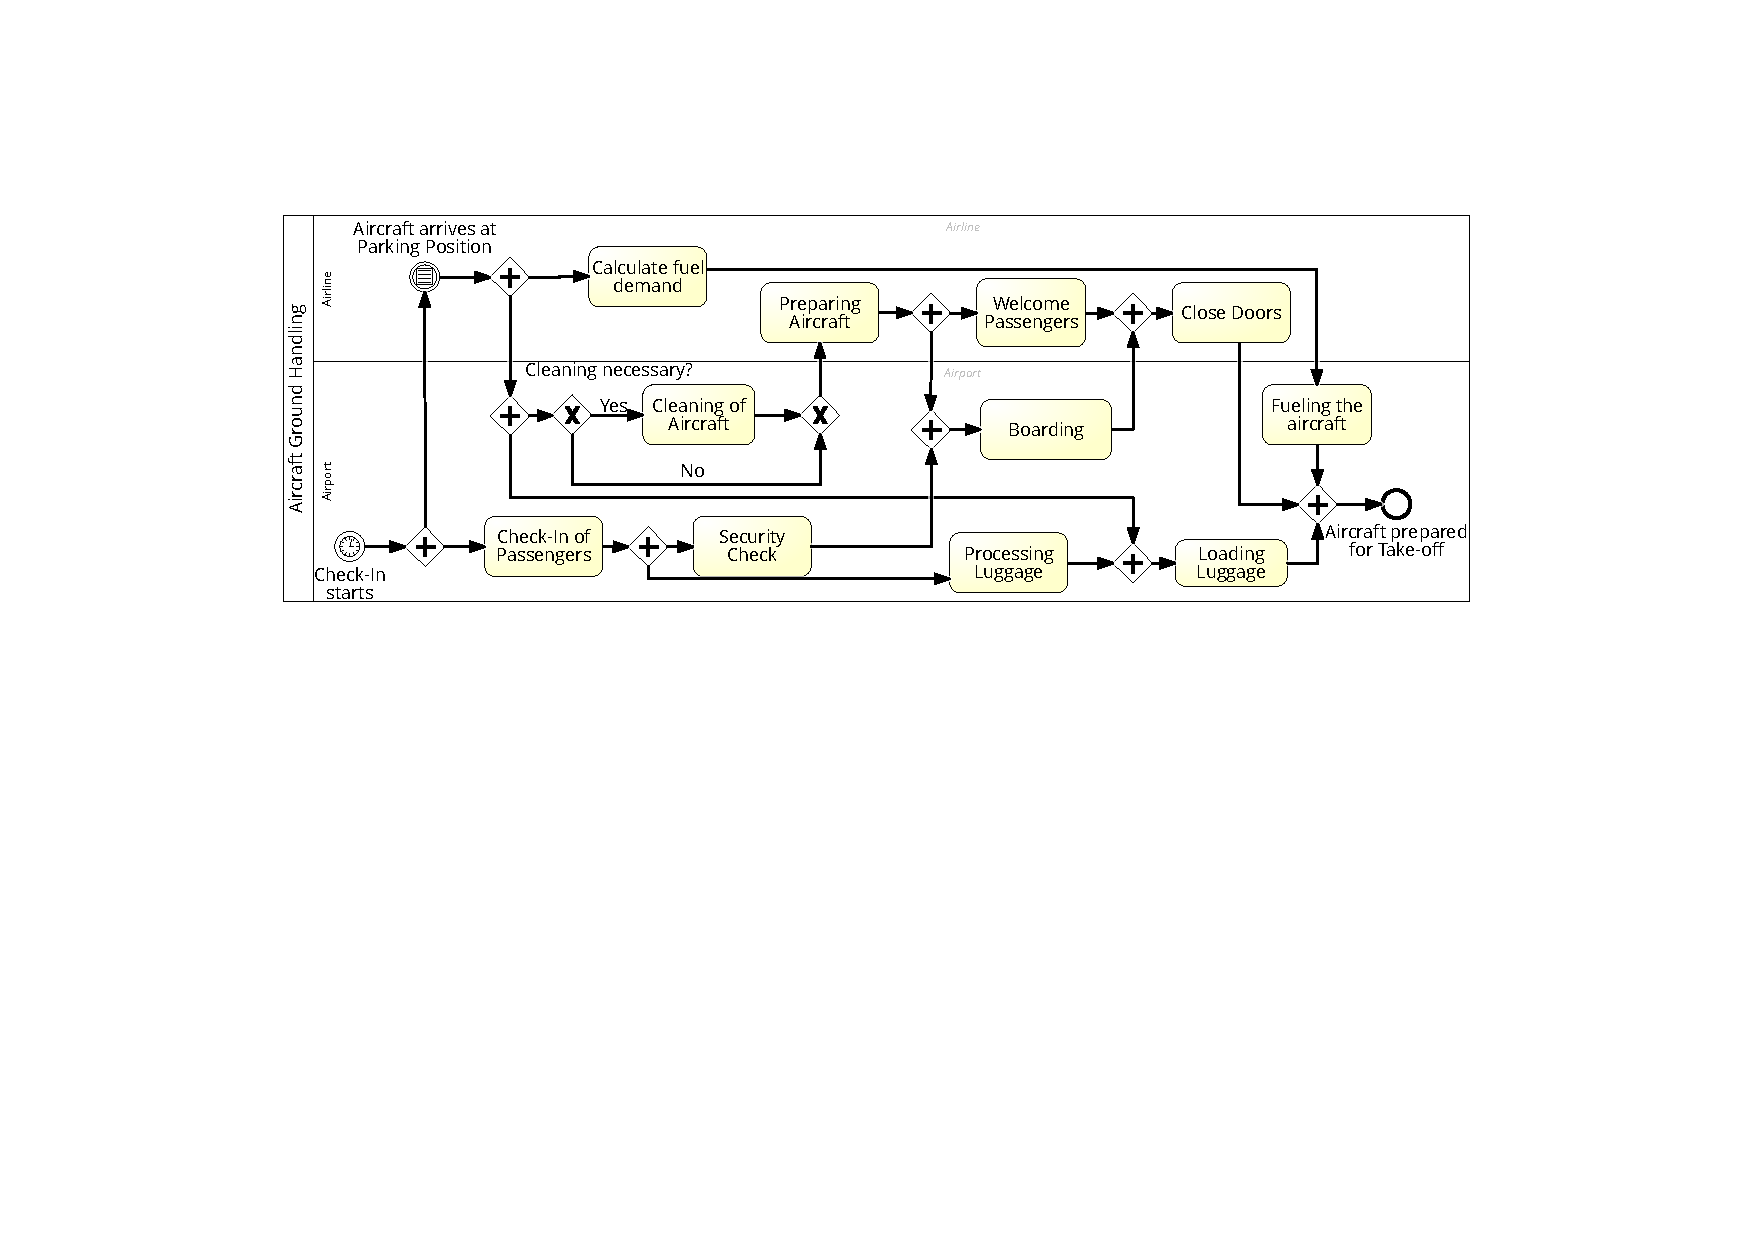
\includegraphics[width=0.98\textwidth]{figures/aircraft_ground_handling_process}
	\caption{The example of an aircraft ground handling process.}
	\label{fig:ground_handling_process}	
	\vspace{-.6em}
\end{figure}


Due to confidentiality issues and privacy regulations, such as GDPR, it is not 
possible for organizations to share their process data with each 
other~\cite{gdpr}. 
Exchanging event logs could reveal personal information of customers or expose 
business secrets. As a consequence, common techniques for process mining cannot 
be employed for inter-organizational business processes, despite the fact that 
these processes can have a large impact of the core operation of a business.
For the aforementioned scenario, for instance, it is well-known that the 
orchestration of ground handling activities is of crucial importance for both 
involved parties~\cite{schmidberger2009ground}. It determines the number of 
flights an airport can operate as well as the number of flights an airline can 
offer per aircraft. 

%Therefore, they lack this powerful tool, if the industry 
%tries to optimize these cross-organizational processes, since process mining 
%is 
%based on the analysis of so called  event logs. Datasets  that contain the 
%data 
%recorded while executing the business process. Nonetheless 
%cross-organizational 
%processes can have a high impact of the core operation of a business, such as 
%the ground handling of an aircraft is essential\cite{schmidberger2009ground} 
%for the number of flights an airport can operate. Therefore, the lack of 
%possibility to apply process mining techniques to cross-organizational 
%business 
%processes is undesirable.

%we are going to introduce a technique to enable organizations to analyse their 
%cross-organizational business processes\cite{van2011intra} without the 
%necessity to share their private data or the need of a trusted third party. 

In this paper, we focus on the question of how to enable process mining for 
inter-organizational business processes without requiring the involved parties 
to share their private event logs or trust a third party.
To this end, we propose an architecture for process mining based 
on \emph{secure multi-party computation}~(MPC)~\cite{yao1982protocols}. In essence, MPC aims 
at the realization of some computation over data from multiple parties, while
exposing only the result of the computation, but keeping the input data 
private. 
%While only enabling the input parties to gain knowledge about the public 
%outputs of the computation. 
We consider the setting of an MPC platform where the 
involved parties upload their event logs to a network of compute nodes. 
Before the upload, secret sharing algorithms locally 
split each single data value into different parts (i.e., shares) that are then 
stored at different nodes. Since each share does not provide any 
information about the original data, the uploaded event log is encrypted and 
exposed neither to the platform operator nor other involved parties. 
Nonetheless, the MPC platform enables the computation over the encrypted data 
through protocols for result sharing among the nodes. 

We realise the above architecture to answer analysis queries that are common in 
process mining. That is, we show how to construct a time-annotated 
directly-follows graph that serves as a starting point for process discovery 
algorithms~\cite{augusto2018automated} and the detection of performance bottlenecks~\cite{van2011time}. We 
implement our proposed architecture using the Sharemind 
platform~\cite{bogdanov2008sharemind}. In order to avoid scalability issues 
that would be imposed by a naive implementation, we employ vectorization of 
event logs and propose a divide-and-conquer scheme for parallel 
processing of sub-logs. We demonstrate the effectiveness of these optimisations 
in an experimental evaluation with real-world event logs. 

The remaining paper is structured as follows. \autoref{sec:background} lays out 
related work and the background for this work. \autoref{sec:approach} 
introduces our architecture for privacy-preserving inter-organizational process 
mining along with the optimizations needed for efficient implementation. An 
experimental evaluation is presented in \autoref{sec:evaluation}, before 
\autoref{sec:conclusion} concludes the paper. 

